%%%%%%%%%%%%%%%%%%%%%%%%%%%%%%%%%%%%%%%%%%%%%%%%%
\chapter{Introducción a los entornos de programación}
\label{ch:intro-prog}
%%%%%%%%%%%%%%%%%%%%%%%%%%%%%%%%%%%%%%%%%%%%%%%%%

%======================================
\section{Antes del editor: cómo escribir su primer programa en un archivo de texto}
\label{sec:plaintext-first}
%======================================

Un programa de Python es texto plano almacenado en un archivo con la
extensión \texttt{.py}. Cualquier herramienta que guarde texto plano (no
texto con formato) puede crear uno. Antes de utilizar un editor
sofisticado, usted creará y ejecutará un programa empleando el editor
de texto más simple disponible en su sistema. Esto establece una idea
fundamental: el editor es irrelevante; lo que importa es el archivo.

\begin{table}[htbp]
\centering
\caption{Cómo abrir un editor de texto plano en cada sistema operativo.}
\label{tab:text-editors}
\begin{tabular}{p{2.8cm} p{5.5cm} p{6.5cm}}
\toprule
\textbf{Sistema operativo} & \textbf{Cómo abrir el editor} & \textbf{Paso crítico antes de escribir} \\
\midrule
Windows &
Presione \texttt{Win + R}, escriba \texttt{notepad} y presione Enter &
En el diálogo Guardar como, establezca «Guardar como tipo» en \texttt{Todos los archivos (*.*)} antes de guardar; de lo contrario, el archivo se guardará como \texttt{hello.py.txt} \\
\midrule
macOS &
Abra Spotlight (\texttt{Cmd + Space}), escriba \texttt{TextEdit} y presione Enter &
Vaya a \textbf{Formato $>$ Convertir en texto simple} antes de escribir cualquier cosa; TextEdit utiliza texto enriquecido de manera predeterminada, lo cual corrompe el código \\
\midrule
Linux &
Presione \texttt{Ctrl + Alt + T} para abrir una terminal; luego escriba \texttt{gedit \&} y presione Enter &
No se requiere ningún paso adicional; \texttt{gedit} guarda texto plano de manera predeterminada \\
\bottomrule
\end{tabular}
\end{table}

\begin{infobox}[title=Ejercicio P-1: Su primer programa de Python]
Escriba el programa que aparece abajo exactamente como se muestra en
su editor de texto. Preste atención a la indentación: los espacios
antes de \texttt{print(n)} y \texttt{if n == 5:} no son decorativos;
son sintaxis de Python obligatoria y el programa fallará sin ellos.
Guarde el archivo como \texttt{hello.py} en una carpeta que pueda
encontrar (su Escritorio es una buena opción). Aplique el paso crítico
de la Tabla~\ref{tab:text-editors} correspondiente a su sistema
operativo antes de guardar.

\begin{warningbox}[title=Los procesadores de texto no son editores de texto]
Microsoft Word, Google Docs y LibreOffice Writer guardan archivos con
marcado de formato invisible. Un archivo de Python guardado con una de
estas herramientas no podrá ejecutarse. Utilice únicamente los
editores listados en la Tabla~\ref{tab:text-editors} o VSC.
\end{warningbox}

\begin{lstlisting}[language=Python]
# Los comentarios comienzan con el caracter #
# Los comentarios no forman parte del programa.
# Pueden usarse para introducir marcadores visuales para mayor claridad
# ----------------------------------------------
# Este programa ejemplifica entrada-salida (I/O),
# bucles, condicionales y asignacion
print("This is programming!")
k = 10
for n in range(k):
    print(n)
    if n == 5:
        print("here")
\end{lstlisting}

La línea \texttt{\#} es un comentario; Python la ignora. Los
comentarios existen para los humanos. \texttt{k = 10} es una
asignación; crea una variable llamada \texttt{k} y almacena el valor
10. \texttt{for n in range(k):} es un bucle; todo lo indentado debajo
se ejecuta 10 veces. \texttt{if n == 5:} es un condicional; el bloque
indentado debajo solo se ejecuta cuando la condición es verdadera.
\end{infobox}

El programa existe como un archivo, pero no hace nada hasta que sea
ejecutado por el intérprete de Python. Ahora que usted ha completado
el Capítulo~\ref{ch:cli-scripting}, dispone de todas las herramientas
necesarias para ejecutarlo. Abra una terminal, navegue hasta la
carpeta donde guardó \texttt{hello.py} y ejecute:

\begin{verbatim}
python hello.py
\end{verbatim}

En macOS y Linux, podría ser necesario utilizar \texttt{python3} en
lugar de \texttt{python}. La salida debería coincidir con lo que
usted esperaría al leer el código.

%======================================
\section{Introducción}
%======================================

Existe una gran cantidad de lenguajes de programación. Para los fines de la computación científica, distinguiremos dos familias principales de lenguajes: lenguajes compilados frente a lenguajes de scripting. Representan dos paradigmas distintos en el diseño de lenguajes de programación, cada uno con sus propias ventajas y compensaciones. La diferencia clave radica en cuándo y cómo el código fuente que usted escribe se traduce a código de máquina que la computadora puede entender y ejecutar.

En el ámbito de la computación científica, la elección entre utilizar un lenguaje compilado como C++ y un lenguaje de scripting como Python a menudo depende de las particularidades del proyecto en cuestión, incluyendo su complejidad, la velocidad de ejecución requerida y la necesidad de acceso directo al hardware.

%======================================
\subsection{Lenguajes compilados}
%======================================

Los lenguajes compilados son aquellos en los que el código fuente se traduce íntegramente a código de máquina antes de la ejecución. Esta traducción la realiza un compilador, un programa que toma todo el código fuente como entrada y genera un archivo ejecutable. Ejemplos de lenguajes compilados incluyen C++, Java, Rust, Go y Swift.

Los lenguajes compilados ofrecen varios beneficios importantes, entre ellos:

\begin{itemize}
	\item Rendimiento: dado que el código está precompilado a código de máquina, los programas compilados suelen ejecutarse más rápido y de manera más eficiente que los interpretados.
	\item Verificación de tipos: muchos lenguajes compilados poseen sistemas de tipos estrictos, los cuales detectan numerosos errores relacionados con tipos en tiempo de compilación, antes de que el código se ejecute.
	\item Seguridad: el código fuente no se distribuye con el software, lo que dificulta que terceros realicen ingeniería inversa del software.
\end{itemize}

Sin embargo, los lenguajes compilados también presentan algunas desventajas:

\begin{itemize}
	\item Velocidad de desarrollo: el ciclo editar-compilar-ejecutar puede consumir mucho tiempo, particularmente en proyectos de software de gran tamaño.
	\item Portabilidad: el ejecutable generado suele ser específico para un tipo de procesador y sistema operativo. La disponibilidad para diferentes sistemas operativos o procesadores podría requerir modificaciones específicas del código fuente y compilaciones independientes.
\end{itemize}

Los lenguajes compilados como C++ se traducen a código de máquina antes de la ejecución, lo que los hace muy rápidos porque son ejecutados directamente por el hardware de la computadora. Esto puede ser una ventaja significativa al tratar con conjuntos de datos enormes o cuando la velocidad de cómputo es un factor crítico.

Sin embargo, la sintaxis de lenguajes como C++ es más compleja y puede requerir más líneas de código para lograr el mismo resultado que un lenguaje de scripting. Además, C++ carece de muchas de las funcionalidades incorporadas de análisis de datos que se encuentran en lenguajes como Python, MATLAB o R, por lo que es necesario utilizar bibliotecas externas como Eigen o Armadillo para operaciones matriciales y otros cómputos complejos.

%======================================
\subsection{Lenguajes de scripting}
%======================================

Los lenguajes de scripting, por otro lado, son típicamente interpretados de texto a instrucciones de máquina, línea por línea de código, justo a tiempo para la ejecución. Si bien esto puede hacer que los lenguajes de scripting sean más lentos que los lenguajes compilados, a menudo son más fáciles de escribir y leer debido a su sintaxis de alto nivel. Ejemplos de lenguajes de scripting incluyen Python, MATLAB, R, JavaScript, Ruby y PHP.

Los lenguajes de scripting ofrecen varias ventajas:

\begin{itemize}
	\item Facilidad de uso: los lenguajes de scripting suelen ser más fáciles de aprender y usar. Tienen una sintaxis menos verbosa y más funcionalidad incorporada.
	\item Flexibilidad: como se interpretan línea por línea, es más fácil realizar cambios en su código y ver su efecto inmediatamente sin tener que recompilar.
	\item Portabilidad: el mismo script puede ejecutarse en cualquier sistema que tenga instalado el intérprete correcto, sin necesidad de cambiar el código.
\end{itemize}

Entre las desventajas de los lenguajes de scripting se encuentran cuestiones relacionadas con:

\begin{itemize}
	\item Rendimiento: los lenguajes interpretados son generalmente más lentos que los lenguajes compilados debido a la sobrecarga de interpretar código línea por línea durante la ejecución.
	\item Dependencia del intérprete: el código solo puede ejecutarse en sistemas que tengan instalado el intérprete correcto.
\end{itemize}

Python es particularmente adecuado para la ciencia de datos biomédicos porque cuenta con numerosas bibliotecas poderosas para el análisis de datos (como Pandas, NumPy y SciPy) y la visualización (como Matplotlib y Seaborn). Además, la sintaxis simple y directa de Python lo convierte en una excelente opción para la creación rápida de prototipos y el análisis exploratorio de datos.

Cabe señalar que, incluso con todos los beneficios de Python, la sintaxis simplificada de MATLAB para operaciones matriciales facilita el desarrollo de algoritmos, ya que el código fuente se asemeja estrechamente a la notación matemática.

%======================================
\subsection{Ejemplos comparativos}
%======================================

Consideremos un ejemplo sencillo en el que deseamos multiplicar dos matrices A y B. Los ejemplos en cada lenguaje se listan abajo en orden alfabético por el nombre del lenguaje.

En C++:
\lstinputlisting[language=C]{../source/IntroProgMatMul.c}

En MATLAB:

\lstinputlisting[language=MATLAB]{../source/IntroProgMatMul.m}

En R:
\lstinputlisting[language=R]{../source/IntroProgMatMul.r}

En Python:
\lstinputlisting[language=Python]{../source/IntroProgMatMul.py}

Del ejemplo anterior, queda claro que el código en MATLAB es mucho más conciso y fácil de comprender que el de C++. Sin embargo, si estuviéramos tratando con matrices muy grandes o necesitáramos realizar esta operación muchas veces en un bucle, el código en C++ podría ejecutarse con mayor rapidez debido a ser un lenguaje compilado.

%In summary, while C++ can offer performance advantages in some circumstances, Python's simplicity, readability, and extensive data-centric libraries make it the language of choice for many data analytics tasks. However, it's worth noting that the right tool should always be chosen based on the specifics of the project and the requirements of the task.

%======================================
\subsection{¿Qué es Python?}
%======================================

Python es un lenguaje de programación \textit{interpretado} y de \textit{alto nivel} para computación de propósito general.

\begin{itemize}
	\item{} \textit{Interpretado} significa que un programa en Python debe ser decodificado línea por línea por otro programa llamado intérprete de Python y traducido a algo que una computadora pueda comprender.
	\item{} \textit{Alto nivel} significa que existe una fuerte abstracción de los elementos del hardware de la computadora; por ejemplo, la memoria no necesita ser preasignada en Python para crear una matriz, mientras que el lenguaje C (un lenguaje de bajo nivel) sí lo requiere. Puede pensar en el nivel del lenguaje como cuán cercanas están las instrucciones al metal de la máquina.
	\item{} El proceso de interpretación del lenguaje se denomina \textit{compilación}, es decir, la traducción de un lenguaje de computadora a otro lenguaje. Esto podría ocurrir múltiples veces hasta que las instrucciones se reduzcan a un lenguaje llamado \textit{assembler} o \textit{ensamblador}; este código coincide estrechamente con la arquitectura de la computadora que ejecuta el programa. Por ejemplo, los programas en Java se compilan a un lenguaje llamado Java bytecode, el cual la Máquina Virtual de Java traduce a ensamblador.
\end{itemize}


%======================================
\subsection{Instalación de Python}
%======================================

Remítase ahora al Capítulo~\ref{ch:environment-setup} para ver las
instrucciones completas de instalación de Python, Visual Studio Code y
todas las herramientas requeridas.

Al ser un lenguaje interpretado, significa que Python requiere un \textit{intérprete}. Esto es lo que usted instala cuando «\textit{instala Python}». Un programa de Python es simplemente un archivo de texto que contiene instrucciones que el intérprete puede entender una línea (o bloque de líneas) a la vez. Puesto que Python es de código abierto, tiene muchos contribuidores; esto resulta en un ecosistema robusto, pero la desventaja es que existen numerosas bibliotecas de software que deben instalarse mientras se rastrea una compleja red de codependencias. Por ello, hay cierta dificultad en instalar un entorno de Python funcional para realizar análisis cuantitativo.

%Anaconda is a Python \textit{distribution}. This means that there is a program with a command line interface and a Graphic User Interface (GUI) that simplifies installation and maintenance of the Python environment. The Anaconda navigator allows users to find and install multiple components, while ensuring that all libraries can still interoperate.

Una manera sencilla de usar el lenguaje Python es a través de un \textit{Entorno de Desarrollo Integrado}. Existen muchos IDE que pueden ejecutar código de Python. Estar familiarizado con más de un entorno es importante, ya que cada uno tiene fortalezas y debilidades. Además, es común que los programas de Python parezcan fallar en un entorno pero funcionen correctamente en otro; esto, por supuesto, es una cuestión de configuración, pero puede ser fuente de frustración ante la falta de conciencia de las fuentes potenciales de conflictos en el software. Particularmente, usted desea saber cómo utilizar herramientas frecuentemente empleadas en el desarrollo de software y necesita exposición a las múltiples opciones que encontrará en la academia, el gobierno y la industria.


%======================================
\subsection{Ejecución de comandos en Python}
%======================================

Los comandos en Python distinguen entre mayúsculas y minúsculas, es decir, usted debe respetar el uso de mayúsculas en las instrucciones tal como aparecen en la documentación. El intérprete de Python ofrece múltiples mecanismos para interactuar con el entorno. El más comúnmente utilizado es la línea de comandos de Python. Puede iniciarla desde un intérprete de comandos. Simplemente escriba {\s python}. El indicador de la línea de comandos cambiará a {\s >>> }

Usted puede ingresar comandos de Python en el indicador de la línea de comandos. Presione \textit{Enter} o \textit{return} para ejecutar comandos. Como la mayoría de los demás lenguajes de programación, Python proporciona expresiones matemáticas. Los bloques de construcción de las expresiones son variables, números, operadores, scripts y funciones.

Las operaciones básicas se listan abajo. \vs

\begin{tabular}{r|l}
\hline
Símbolo 		& Operación \\
\hline
$+$       	&    Adición \\
$-$       	&    Sustracción \\
$\star$   	&    Multiplicación \\
$/$       	&    División \\
$\star\star$&      Potencia \\
\hline
\end{tabular}

\vs

Algunos comandos son como los que uno escribiría en una calculadora. Si usted desea hacer referencia al resultado del comando, necesita asignarle un nombre, o en otras palabras, asignar el resultado a una variable. El siguiente comando asigna el resultado a la variable s. (Observe que Python no guardó la respuesta verdadera 7/12, sino una aproximación decimal.)

\begin{lstlisting}[language=Python]
>>> s = 1/3 + 1/4
\end{lstlisting}

Si desea saber qué contiene la variable $s$, simplemente escriba su nombre en el indicador de comandos:

\begin{lstlisting}[language=Python]
>>> s
0.5833333333333333
\end{lstlisting}

Si un comando no cabe en una sola línea, utilice una barra invertida (\textbackslash) seguida de Return/Enter para indicar que la sentencia continúa en la línea siguiente. Por ejemplo,

\begin{lstlisting}[language=Python]
>>> s = 1 - 1/2 + 1/3 -1/4 + 1/5 - 1/6 + 1/7 \
... :- 1/8 + 1/9 - 1/10 + 1/11 - 1/12
\end{lstlisting}

Escriba $s$ y presione Enter para ver el nuevo valor de $s$.

\begin{lstlisting}[language=Python]
>>> s
0.6532106782106782
\end{lstlisting}

Utilice el doble asterisco ($**$) para elevar algo a un exponente.

\begin{lstlisting}[language=Python]
>>> 89**2
7921
\end{lstlisting}

Los números imaginarios pueden utilizarse con la constante $j$, que representa $\sqrt{-1}$ de forma predeterminada.

\begin{lstlisting}[language=Python]
>>> (1j)**2
(-1+0j)
\end{lstlisting}

Por lo tanto, usted debe tener cuidado al utilizar la variable $j$ cuando trabaje con números complejos. ¿Qué espera de la siguiente operación? ¿Puede explicar lo que observa? Quizás necesite completar el capítulo entero antes de poder responder esta pregunta. \QA

\begin{lstlisting}[language=Python]
>>> j = 10
>>> j = j*(-1)**(0.5)
>>> j
\end{lstlisting}

¿El resultado almacenado en la variable {\s j} coincide con su expectativa? Explique. \QA

Python utiliza notación decimal convencional, con un punto decimal opcional y un signo más o menos inicial, para los números. La notación científica utiliza la letra e o E para especificar un factor de escala de potencia de diez. Los números imaginarios utilizan i como sufijo. (Este curso no utiliza números complejos, pero usted podría generar errores con alguno de ellos.)

Algunos ejemplos de números válidos son: 1, -1, 0.0001, 9.87654321, 1.2345e10, 1.2345*10**10, 1j, -2j, 3e5j.

Al asignar nombres a variables o expresiones, es una buena práctica hacer que los nombres sean útiles. Por ejemplo, en el segundo comando anterior, le dimos al resultado el nombre rhoSq para implicar «rho al cuadrado». Observe que {\bf NO PUEDE} tener espacios en los nombres de las variables (es decir, sin espacios en los nombres del lado izquierdo del signo igual). Dar nombres útiles a sus variables o salidas le ayudará a llevar un registro de lo que está haciendo.

%We will have another lab in which we will address programming standards and source control, an area technically known as \textit{configuration management}.

Usted puede utilizar las teclas de flecha arriba y abajo para recuperar fácilmente un comando y luego editarlo con las flechas izquierda y derecha. Pruébelo. Esta es la manera más rápida de repetir comandos de Python que pudo haber utilizado en el pasado.

%======================================
\subsection{El editor de Python de VSC: ejecución de un programa simple}
%======================================

Descargue el archivo {\s lab1SimpleInstruction.py}. Abra el archivo en VSC. Las siguientes instrucciones aparecerán en el editor:


\begin{lstlisting}[language=Python]
k=0;
for i in range(1,11):
    k=k+1/10;
    print(k)
print(k==1)
\end{lstlisting}

Puede hacer clic en el botón \textit{Run file} de la barra de herramientas (como se muestra en la Figura \ref{fig:VSCFileInst}), o presionar F5. Llamamos a todas estas acciones \textit{ejecutar un programa}. El programa {\s lab1SimpleInstruction.py} suma diez veces el número 0.1. La comparación del número 1 contra la suma devuelve un valor de \textit{false}, mientras que la aritmética elemental nos dice que sumar el número 0.1 diez veces debería resultar en 1, y el valor devuelto debería ser \textit{true}. ¿Por qué este resultado es false? \QA Una vez ejecutado el programa, la parte inferior de VSC muestra un panel etiquetado TERMINAL, así como otras pestañas etiquetadas PROBLEMS, OUTPUT y DEBUG CONSOLE, como se muestra en la Figura \ref{fig:VSCFileInstExec}

\begin{figure}
	\centering
		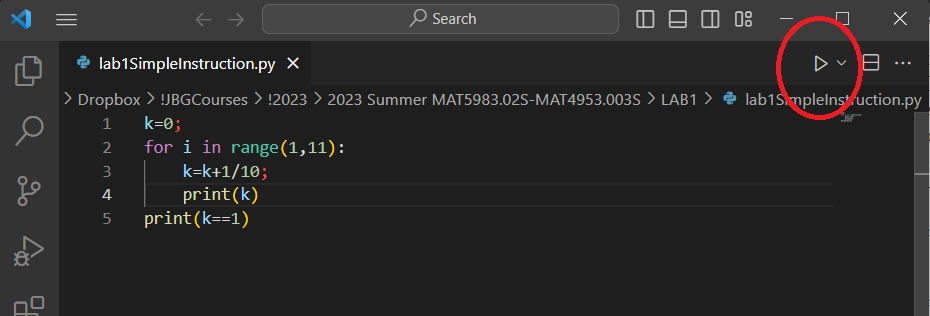
\includegraphics[width=0.7\textwidth]{../images/ChapterIntroProg/VSCFileInst.png}
	\caption{Para ejecutar un archivo de Python en VSC, simplemente haga clic en el botón Run, representado por un triángulo que apunta hacia la derecha. Se ha resaltado con un círculo.}
	\label{fig:VSCFileInst}
\end{figure}


\begin{figure}
	\centering
		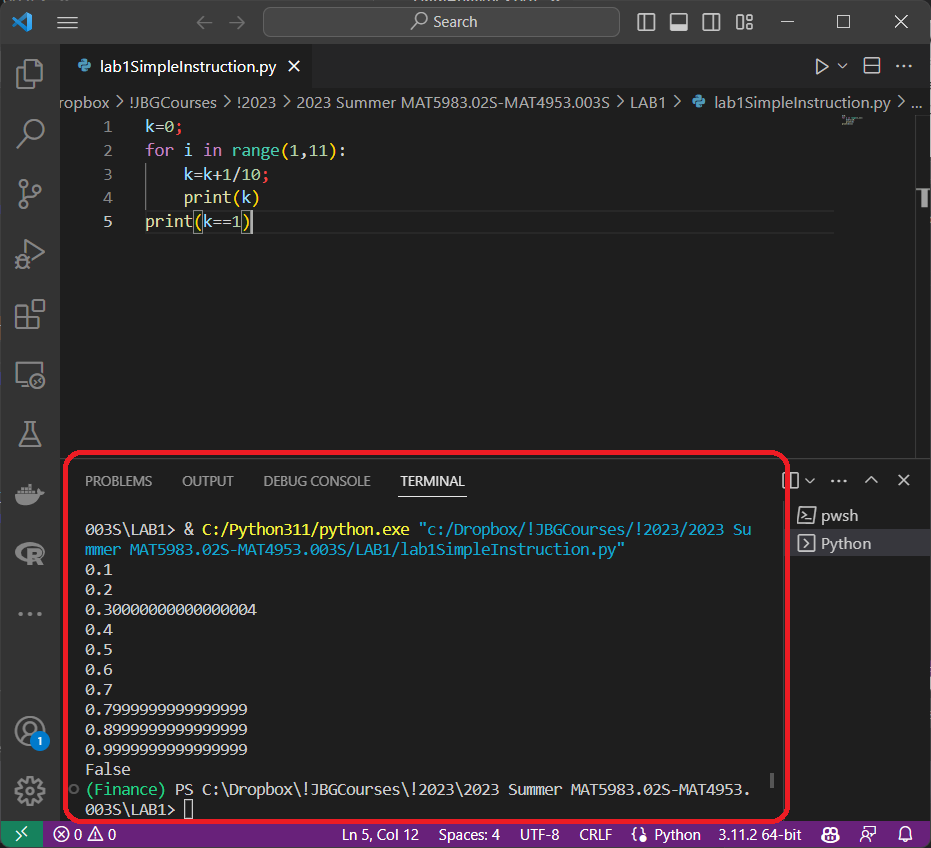
\includegraphics[width=0.7\textwidth]{../images/ChapterIntroProg/VSCFileInstExec.png}
	\caption{Ejecutar un programa de Python activa la línea de comandos. Los resultados se imprimen en ese panel. La línea de comandos se resalta con un recuadro redondeado.}
	\label{fig:VSCFileInstExec}
\end{figure}

Observe que usted puede ingresar comandos en la terminal. Por ejemplo, escriba {\s 1+1} y presione Enter. Pruebe operaciones matemáticas como raíz cuadrada o funciones trigonométricas. ¿Qué retos encuentra? \QA

En el programa {\s lab1SimpleInstruction.py} todas las líneas de código se ejecutaron secuencialmente, una a la vez. Esto es lo que llamamos un \textbf{archivo de script}. Es decir, cuando usted ejecuta un archivo de script, espera que ocurra algo tangible, ya sea un mensaje en pantalla, un archivo alterado, una comunicación que tiene lugar, etc.

Existe una forma de utilizar archivos de código fuente para mantener código que se ejecutará más tarde, sin necesariamente ejecutar ninguna instrucción. En este punto, abra el archivo {\s lab1Function.py}. Verá las siguientes instrucciones:

\begin{lstlisting}[language=Python]
def sum1(n):
    # sum1(n) calcula la suma de 1 + 2 + ... + n
    total = 0;
    for i in range(1,n):
        total = total + i
    return total
\end{lstlisting}

Este archivo define una función llamada {\s sum1(n)}. El comando {\s sum(3)} devuelve 6 puesto que
$1 + 2 + 3 = 6$. Es instructivo ver cómo este código realiza su trabajo.
\begin{itemize}
	\item La instrucción {\s def} indica el comienzo de una \textit{función}. Observe que todas las instrucciones que se ejecutan dentro de esa función tienen una alineación vertical desplazada hacia la derecha para indicar que todos estos comandos están subordinados a {\s def}. Este desplazamiento en la alineación vertical se denomina indentación. Es parte de la sintaxis del lenguaje de programación Python; por lo tanto, siempre debe tratar las indentaciones de manera estricta.
	\item La instrucción {\s \# sum1(n)...} es un \textit{comentario}. Las líneas de código que comienzan con el símbolo {\s \#} no se ejecutan. El punto y coma al final es opcional.
	\item La instrucción {\s total = 0;} es una \textit{asignación}. Esta línea de código crea la variable {\s total} y le asigna el valor cero.
	\item La instrucción {\s for i in range(1,n):} inicia un \textit{bucle}. Las instrucciones subordinadas, identificadas por indentación, se repetirán $n$ veces. Particularmente, la instrucción {\s range(1,n)} crea una secuencia de enteros que comienzan en 1 y terminan en $n$. ¿Cuál es el resultado de {\s range(10,13)}?
	\item La instrucción {\s total = total + i} es una asignación. Es muy importante enfatizar que esto no es una ecuación; si lo fuera, {\s total} se cancelaría e {\s i} sería cero. Lo que ocurre es que por cada repetición del bucle, la variable {\s total} se redefine para contener su valor anterior más el valor de {\s i}.
	\item La instrucción {\s return total} es la salida de la función. Es decir, si de alguna manera pudiéramos ejecutar esta función como {\s x = sum1(3)}, la variable {\s x} contendría el valor 6, puesto que {\s sum1(3)} $= 1 + 2 + 3 = 6$.
\end{itemize}

Ahora modificaremos este archivo. Agregue al final un programa llamado {\s sum2} en el cual sumemos enteros elevados al cuadrado. La siguiente pregunta debe ser: ¿cómo ejecutamos estas funciones?

El comando {\s python [filename]} puede utilizarse para ejecutar un programa de Python desde la terminal, o desde cualquier indicador de línea de comandos. Pero si ejecutamos lo siguiente en el indicador de comandos, no ocurre nada:

\begin{lstlisting}[language=Python]
	python lab1Function.py
\end{lstlisting}

¿Por qué? \QA

Ahora, agregue la siguiente línea de código al final del archivo, \textbf{sin indentación}:

\begin{lstlisting}[language=Python]
print(sum1(2))
\end{lstlisting}

Ejecute el programa. ¿Cuál fue el resultado de {\s sum1(2)}? ¿Es esto lo que esperaba? ¿Por qué? \QA Calcule a mano cuál debería ser la salida de {\s sum1(3)}. Ahora cambie la última línea del programa para que lea {\s print(sum1(2))}

Lo que hicimos fue simplemente definir una función y luego utilizarla. Observe que si usted coloca la línea de código anterior al inicio del archivo, el intérprete de Python lanzaría una excepción porque la función {\s sum1} aún no es conocida por el intérprete... tenga presente que el intérprete de Python ejecuta una línea de código a la vez en orden secuencial (quizás con ramificaciones y repetición, como exploraremos más adelante). Por lo tanto, las funciones deben definirse antes de que puedan invocarse dentro de un archivo.

¿El programa {\s } produjo el resultado que usted esperaba? En caso de que no lo hiciera, ingrese la siguiente instrucción en la terminal: {\s man range}. Este comando muestra el manual ({\s man}) para la función {\s range}. El hecho de que {\s range} se comporte de ciertas maneras no lo obliga a usted a regirse por ese diseño en particular. De hecho, usted puede modificar {\s sum1} de modo que el resultado corresponda a lo que un usuario ingenuo esperaría. Para lograrlo, necesitará cambiar el límite de range dentro de la función. Impleméntelo y explique. \QA

%======================================
\subsection{Ejecución de funciones}
%======================================

En la sección anterior, agregamos una sola línea de código al final del programa para calcular la función que programamos. Sin embargo, existe un caso de uso más interesante: crear una función que otros programas puedan reutilizar. Para utilizar una función existente desde un archivo, debemos importar esa función al entorno de Python. Ya hicimos algo así cuando importamos NumPy.

Ahora importaremos la función {\s sum1} desde el archivo {\s lab1Function.py}. Para ello, ejecute el siguiente comando:

\begin{lstlisting}[language=Python]
	import lab1function as LAB1
\end{lstlisting}

Esta instrucción carga en memoria un directorio de todas las funciones presentes en ese archivo. Ahora usted puede invocar las funciones que creó. Por ejemplo,

\begin{lstlisting}[language=Python]
	LAB1.sum2(3)
\end{lstlisting}

También es posible cargar en memoria una sola función desde un archivo. Podemos lograrlo ejecutando

\begin{lstlisting}[language=Python]
	from lab1function import sum1
\end{lstlisting}

En este caso, no hay alias asociado con la función. Para usarla, usted simplemente puede llamar la función con un parámetro, como en {\s sum2(3)}

Investigue un poco sobre cómo cargar múltiples funciones con una sola instrucción. Explique. \QA

%-----------------------------------------
\section{Introducción a NumPy}
%-----------------------------------------
Las operaciones numéricas pueden programarse en Python. Una biblioteca llamada {\s NumPy} encapsula mucha funcionalidad necesaria y se ha convertido en el estándar \textit{de facto}. El elemento de datos básico en {\s NumPy} es un arreglo multidimensional. Esto le permite resolver muchos problemas de computación técnica, especialmente aquellos con formulaciones matriciales y vectoriales, en una fracción del tiempo que tomaría escribir un programa en un lenguaje de bajo nivel como C.

Por ejemplo, en el indicador de Python escriba el siguiente comando y presione Enter.

\begin{lstlisting}[language=Python]
	import numpy as np
\end{lstlisting}

Este comando carga en memoria una referencia a la biblioteca NumPy. Ahora puede acceder a todas las funciones de esta biblioteca utilizando el prefijo {\s np}; este es un \textit{alias}. Puede elegir cualquier alias que desee, pero es costumbre usar {\s np} para NumPy. Ahora ingrese el siguiente comando:

\begin{lstlisting}[language=Python]
	np.sqrt(9)
\end{lstlisting}

La función {\s sqrt} calcula la raíz cuadrada de un número real. He aquí un ejemplo y los valores resultantes.

\begin{lstlisting}[language=Python]
>>> rho = (1+np.sqrt(5))/2
>>> rhoSq = rho**2
>>> a = rhoSq + rho
>>> a
4.23606797749979
\end{lstlisting}

Sin embargo, usted no puede utilizar la función {\s sqrt} con números negativos. ¿Qué tendría que hacer para permitir que Python calcule la raíz cuadrada de un número negativo y devuelva un número complejo? \QA %So, instead of {\s sqrt(-2)} you will have to use {\s (-2)**0.5}.


La biblioteca NumPy ofrece acceso fácil a constantes de uso común, tales como:

\vs

\begin{tabular}{r|l}
Constante 		& Valor\\
\hline
{\s np.e} 		& Devuelve el número $e$ \\
{\s np.pi} 		& Devuelve el número $\pi$ \\
{\s np.inf} 	& Devuelve el número $\infty$ \\
{\s np.nan} 	& NaN, no-es-un-número \\
\hline
\end{tabular}

\vs

%MATLAB: Infinity is generated by dividing a nonzero value by zero, or by
%evaluating well defined mathematical expressions that overflow.
%(Try $10^{310}$ or $\exp(999)$.)

%MATLAB: Not-a-number is generated by trying to evaluate expressions like
%0/0 or Inf-Inf that do not have well defined mathematical values.

Las expresiones utilizan los operadores aritméticos y reglas de precedencia que usted ya conoce a estas alturas. También existen funciones, como coseno o seno. La entrada a la función se rodea con paréntesis. Con NumPy, ahora podemos acceder a funciones matemáticas de uso común. Entre otras: \vs

\begin{tabular}{r|l}
Función 			& Operación \\
\hline
{\s np.abs(x)} 		& Valor absoluto $|x|$ \\
{\s np.sqrt(x)}		&  Raíz cuadrada $\sqrt{x}$ \\
{\s np.exp(x)} 		& Función exponencial $e^x$ \\
{\s np.log(x)} 		& $\log(x)$ donde $x$ es un número real positivo\\
{\s np.sin(x)}		&  $\sin(x)$ donde se asume que $x$ está en radianes \\
{\s np.cos(x)}		& $\cos(x)$ donde se asume que $x$ está en radianes \\
\hline
\end{tabular}

\vs

La biblioteca NumPy tiene \textit{muchas} funciones. Puede encontrarse una lista exhaustiva en \url{https://numpy.org/doc/stable/reference/}. Ahora ingrese el siguiente comando:

\begin{lstlisting}[language=Python]
	x = np.random.standard_normal(3)
\end{lstlisting}

No hay salida. ¿Por qué cree usted que este es el comportamiento? \QA En el lado derecho de la ventana de Spyder hay una pestaña llamada \textit{Variable Explorer}. Esta mostrará el valor de $x$. Alternativamente, puede ingresar

\begin{lstlisting}[language=Python]
	print(x)
\end{lstlisting}

De manera alternativa, puede imprimir el resultado directamente sin asignarlo a una variable. Pruebe

\begin{lstlisting}[language=Python]
	print(np.random.standard_normal(3))
\end{lstlisting}

¿Por qué los resultados de esta última operación son diferentes de los valores almacenados en la variable $x$? \QA



%-----------------------------------------
\subsection{Operaciones matriciales}
%-----------------------------------------

El elemento de datos básico en NumPy es un arreglo multidimensional.
A veces se le atribuye un significado especial a las matrices de 1 por 1, que se
denominan escalares, y a las matrices con una sola fila o columna, las cuales
se denominan vectores. Python tiene otras formas de almacenar datos tanto
numéricos como no numéricos, pero al principio, normalmente es mejor
pensar en todo como una matriz.

Los vectores fila se delimitan en notación por corchetes. Una coma separa los números individuales en un vector fila. Múltiples vectores fila del mismo tamaño se separan por comas y se delimitan con corchetes para definir una matriz. Es práctica común utilizar una letra mayúscula al nombrar matrices con el fin de distinguirlas de un vector, escalar o valor de variable individual.

Ahora, crearemos un vector y una matriz para demostrar operaciones matriciales simples \vs

{\footnotesize
\begin{tabular}{r|l}
Función 						& Operación \\
\hline
{\s x = np.array([1,2,3,4])} 	&   Crea el vector fila $\x = [1,2,3,4]$\\
{\s b = np.array([1,2,3])}		&   Crea el vector fila $\bb = [1,2,3]$\\
{\s A = np.array([[1,2,3],[4,5,6],[7,8,9]])}  			&   Crea la matriz $ A = \begin{bmatrix} 1 & 2 & 3\\ 4 & 5 & 6 \\ 7 & 8 & 9 \end{bmatrix} $\\
{\s B = np.ones([2,3])}   		&   Crea la matriz $ A = \begin{bmatrix} 1 & 1 & 1\\ 1 & 1 & 1 \end{bmatrix} $\\
{\s C = np.zeros([2,3])}   		&   Crea la matriz $ A = \begin{bmatrix} 0 & 0 & 0\\ 0 & 0 & 0 \end{bmatrix} $\\
\hline
\end{tabular}
}

\vs
Los siguientes comandos demuestran casos básicos de manipulación de vectores:
\vs

\begin{tabular}{r|l}
Operación 	& Resultado \\
\hline
{\s x[-1]} 	&   Devuelve 4, el último elemento de $x$\\
{\s x[1]} 	&   Devuelve 2, el segundo elemento de $x$\\
{\s x[-2]} 	&  Devuelve 3, el penúltimo elemento de $x$\\
\hline
\end{tabular}

\vs
El operador dos puntos (:) es notable. En notación vectorial, indica un rango de filas o columnas. En Python, el primer elemento de un vector tiene índice 0; el segundo elemento tiene índice 1, y así sucesivamente. El operador dos puntos $a:b$ comienza en la fila o columna de índice $a$ y cubre hasta un índice menor que $b$. Así, $A[0:2,0:2]$ devuelve una matriz compuesta por las filas 1 a 2 y las columnas 1 a 2 con respecto a la matriz $A$.

Los siguientes comandos demuestran casos básicos de manipulación de matrices:
\vs

\begin{tabular}{r|l}
Operación 			& Resultado \\
\hline
{\s A[1,2]} 				&  Valor de la $2^{da}$ fila y $3^{ra}$ columna de $A$\\
{\s A[0:2,0:2]} 		&  Devuelve $A = \begin{bmatrix} 1 & 2 \\ 4 & 5\end{bmatrix} $\\
{\s A[1:3,1:3]} 		&  Devuelve $A = \begin{bmatrix} 5 & 6 \\ 8 & 9\end{bmatrix} $\\
%$A[1:100,1:100]$ 		&  Returns $A = \begin{bmatrix} 5 & 6 \\ 8 & 9\end{bmatrix} $\\
\hline
\end{tabular}

\vs

La matriz $A$ tiene tres filas y tres columnas. Entonces, ¿por qué $A[1:100,1:100]$ no produce un error? \QA

El tamaño o dimensión de una matriz se refiere al número de filas y
número de columnas que tiene una matriz. El comando {\s shape} devuelve el número
de filas y columnas de una matriz.
Observe que el resultado es un vector: una matriz unidimensional con
2 valores, donde el primero es el número de filas y el segundo valor
es el número de columnas. Al acceder a cada elemento de este vector,
podemos acceder a cada dimensión de manera individual.

Utilizando la matriz $A$ de nuestros ejemplos anteriores,

\begin{lstlisting}[language=Python]
>>> y = A.shape()
>>> y
(3,3)
>>> y[0]
3
>>> y[1]
3
\end{lstlisting}

El siguiente ejemplo ilustrará una sutileza en la copia de matrices:

\begin{lstlisting}[language=Python]
>>> D = A

array([[1, 2, 3],
       [4, 5, 6],
       [7, 8, 9]])
>>> D[0,0] = 9
>>> A

array([[9, 2, 3],
       [4, 5, 6],
       [7, 8, 9]])
\end{lstlisting}

Observe que al actualizar un valor en $D$, el valor correspondiente en $A$ cambió. ¿Por qué? ¿Qué necesitaría hacer para evitar que una actualización en $D$ modifique $A$? \QA

Las operaciones matriciales básicas se listan abajo, usando las matrices de los ejemplos anteriores.
\vs

\begin{tabular}{r|l}
Operación 		& Resultado \\
\hline
{\s$A.T$} 	&  Transpuesta de $A$.\\
{\s$A.conj().T$} 	&  Transpuesta conjugada de $A$.\\
{\s$A@B.T$} 			&  Multiplicación de matrices $A \cdot B$. \\
{\s$A\star A$} 		&  Multiplicación elemento a elemento\\
{\s$A/A$} 		&  División elemento a elemento\\
{\s$A\star\star 2$} 		&  Exponenciación elemento a elemento\\
\hline
\end{tabular}

\vs

NumPy ofrece una manera sencilla de resolver sistemas de ecuaciones lineales. Dada la matriz $A$ y el vector $\bb$ de los ejemplos anteriores, el sistema lineal $A\x = \bb$ puede resolverse invocando {\s np.linalg.solve} de la siguiente manera

\begin{lstlisting}[language=Python]
>>> x = np.linalg.solve(A,b)
array([-0.23333333,  0.46666667,  0.1       ])
\end{lstlisting}

Es fácil utilizar la multiplicación de matrices $A\x$ para comprobar la respuesta

\begin{lstlisting}[language=Python]
>>> A@x
array([1., 2., 3.])
\end{lstlisting}


% %======================================
% \section{Specific tasks for this chapter}
% %======================================

% %-----------------------------------------
% \subsection{Data Challenge Text File}
% %-----------------------------------------
% Refer to the Data Challenge volume for specific information. What follows shows general problems and approaches. We will illustrate this problem with three simple questions: (1) How many school districts were there in total?, (2) How many schools districts were there in Virgina? (3) How many school districts were there in Pensylvannia?

% A common approach to extract information from comma-separated or flat files is by importing it into Excel. The ``\textit{Text Import Wizard}'' would guide you through the process of identifying variables by column.
% %However, this results in a problem. Describe it. \QA
% % \begin{figure}
% % 	\centering
% % 		
\includegraphics{../figures/ChapterIntroProg/Excel.png}
% % 	\caption{Excel's Import Wizard}
% % 	\label{fig:Excel}
% % \end{figure}

% A simple program in Python to help you explore this file is described below:

% \BeginCode
% f = open("LEA Characteristics.csv", "r", encoding="cp1252")
% counter = 0;
% for x in f:
%     counter = counter + 1
% print(counter)
% \end{verbatim}
% \EndCode

% The previous file counts the total number of rows in the file. Does this number coincide with the number produced by Excel? \QA

% The instruction \textit{encoding=``cp1252"} is necessary in non-Windows systems due the presence of single-byte character encoding of the Latin alphabet, used by default in the legacy components of Microsoft Windows for English and many European languages including Spanish, French, and German. If you remove this instruction, the following error might show up in non-Windows operating systems: ``'utf-8' codec can't decode byte...''

% Now, to count the total number of schools in PA, use the following code:


% \BeginCode
% f = open("EDGE_GEOCODE_PUBLICLEA_1718.TXT", "r", encoding="cp1252")
% counter = 0;
% for x in f:
%     y = x.split(',')
%     if x[0] == "PA": # Change for Virgina
%         counter = counter + 1
% print(counter)
% \end{verbatim}
% \EndCode

% Can you explain what this code does?  \QA




%Using this template, try to answer the questions in the assignment. \QA

%Now, create multiple functions in a single file. Each function will test  a single condition and return a Boolean value. At the end of the file, add the code above and modify it to call each function instead of using the position of $x$. So, instead of the code above, you will have something like

% \BeginCode
% f = open("US1969.dat", "r")
% counter = 0;
% for s in f:
%     if isLiveBirth(s) and isTexanMother(s):
%         counter = counter + 1
% print(counter)
% \end{verbatim}
% \EndCode

% The advantage of writing your code like in this example is that the program becomes self-explanatory. Writing clear programs is an invaluable skill to guarantee maintainability, to reduce development time, and to facilitate communication. This skill requires substantial practice.

% %-----------------------------------------
% \subsection{One year of NCHS data}
% %-----------------------------------------
% Since 1969, all births recorded in the US are available as digital records from the National Center for Health Statistics (NCHS) from the Centers for Disease Control and Prevention (CDC). Only between 1969 and 1988 the date and time of birth is publicly available; starting in 1989, only the week of birth is recorded. Why is the date and time of birth no longer recorded? \QA

% Open the file US1969.zip. It contains birth records from 1969, and a data dictionary. The uncompressed data file is about 380 MB in size. The data is contained in a ``flat file''. This means that every line of text in this file is a continuous chain of characters. We must extract information from this type of file with a ``dictionary'' that tells us the beginning and ending columns of a given variable. Why was this format used? \QA

% A common approach to extract information from flat files is by importing it into Excel. The ``\textit{Text Import Wizard}'' would guide you through the process of identifying variables by column. However, this results in a problem. Describe it. \QA
% \begin{figure}
% 	\centering
% 		
\includegraphics{../figures/ChapterIntroProg/Excel.png}
% 	\caption{Excel's Import Wizard}
% 	\label{fig:Excel}
% \end{figure}


% A simple program that can help you explore this file is

% \BeginCode
% f = open("US1969.dat", "r", encoding="cp1252")
% counter = 0;
% for x in f:
%     if x[25] == "7" and x[26] ==  "4": # other conditions?
%         counter = counter + 1
% print(counter)
% \end{verbatim}
% \EndCode

% The instruction \textit{encoding=``cp1252"} is necessary in non-Windows systems due the presence of single-byte character encoding of the Latin alphabet, used by default in the legacy components of Microsoft Windows for English and many European languages including Spanish, French, and German. If you remove this instruction, the following error might show up in non-Windows operating systems: ``'utf-8' codec can't decode byte...''

% %Using this template, try to answer the questions in the assignment. \QA

% Now, create multiple functions in a single file. Each function will test  a single condition and return a Boolean value. At the end of the file, add the code above and modify it to call each function instead of using the position of $x$. So, instead of the code above, you will have something like

% \BeginCode
% f = open("US1969.dat", "r")
% counter = 0;
% for s in f:
%     if isLiveBirth(s) and isTexanMother(s):
%         counter = counter + 1
% print(counter)
% \end{verbatim}
% \EndCode

% The advantage of writing your code like in this example is that the program becomes self-explanatory. Writing clear programs is an invaluable skill to guarantee maintainability, to reduce development time, and to facilitate communication. This skill requires substantial practice. Address plotting, and additional questions in a similar manner.  Turn in your code. \QA

% %-----------------------------------------
% \subsection{Questions for this chapter}
% %-----------------------------------------

% \noindent \textbf{Introductory Level:}
% \begin{enumerate}
% 	\item How many live births occurred in Texas in 1969 from mothers residing in Texas?	\QA
% 	\item How do you know that your answer is correct? \QA
% 	\item Show graphically how the level of education of the mother is related to the birth order (1st born, second child, third, etc.)	\QA
% 	\begin{itemize}
% 		\item Bonus question: Plot births from each state with respect to every other state. \QA
% 	\end{itemize}
% 	\begin{itemize}
% 		\item Bonus question: Plot each variable with respect to every other variable. \QA
% 	\end{itemize}
% \end{enumerate}

% \noindent\textbf{Intermediate Level:}
% \begin{enumerate}
% 	\item How many live births occurred in every state in 1969 from mothers residing in the state where the baby was born?	\QA
% 	\item How do you know that your answer is correct? \QA
% 	\item What variables are \textbf{correlated} with low weight at birth?  \QA  Recall that the {\em Correlation coefficient} between two random
% variables $X$ and $Y$ is defined as $$\rho(X,Y) = \frac{{\bf
% Cov}(X,Y)}{\sqrt{{\bf Var}(X){\bf Var}(Y)}}.$$ The {\em sample
% correlation coefficient} $r$ between two samples $x_i$ and $y_j$ is
% defined as $r = S_{xy}/\sqrt{S_{xx}S_{yy}}.$
% 	\item What variables are correlated with stillbirths? \QA
% \end{enumerate}


